\documentclass[aspectratio=169,xcolor=table]{beamer}
\usepackage{algorithm}
\usepackage{algpseudocode}
\usepackage[utf8]{inputenc}
\usepackage[T1]{fontenc}
\usepackage{lipsum, lmodern}
\usepackage{csquotes}
\usepackage{xcolor}
\usepackage[portuguese]{babel}
\usepackage{booktabs}
\usepackage{amssymb}
\usepackage{textcomp}
\usepackage{url}

% ------------------------------------------------
% Tema e Configurações do Beamer
% ------------------------------------------------
\usetheme{DCC}

% Ajuste de espaçamento entre itens
\setbeamertemplate{itemize items}[circle]
\setbeamertemplate{itemize subitem}[circle]
\setlength{\itemsep}{0.8em}
\setlength{\parskip}{0.5em}

\graphicspath{{imgs/}{./imgs/}{../Imagens/}{../Imagens/telas/}}

\author[Magalhães, Antoniel]{%
  \textbf{Antoniel Magalhães de Sousa}
}
\title{SISDEF 3.0: Modernização e Reengenharia de um Sistema para Gerenciamento de Defesas de TCC}
\subtitle{Reescrita Completa com TypeScript Full-Stack}
\institute{Universidade Federal da Bahia \\ Instituto de Computação}
\date{\today}

\begin{document}

%-------------------------------------------------
%  SLIDE DE TÍTULO
%-------------------------------------------------
\begin{frame}[plain,noframenumbering]
    \titlepage
\end{frame}

%-------------------------------------------------
%  SLIDE DE AGENDA
%-------------------------------------------------
\begin{frame}{Agenda}
    \tableofcontents
\end{frame}

\setlength{\parskip}{1em}

%=================================================
\section{Contexto e Problema}
%=================================================

\begin{frame}{Sistemas de Informação Acadêmicos}
    \begin{itemize}
        \item \textbf{Definição}: Sistema responsável pela coleta, processamento, análise e disseminação de informações
        \item \textbf{Objetivo}: Contribuir para tomada de decisões e suporte a processos organizacionais
        \item \textbf{Contexto Acadêmico}:
        \begin{itemize}
            \item Organização e gestão de atividades
            \item Agilização de processos (comunicação, cooperação, coordenação)
            \item Armazenamento eficiente de dados
            \item Geração de novas informações
        \end{itemize}
    \end{itemize}
\end{frame}

\begin{frame}{O Problema: Gestão Manual de Defesas}
    \textbf{Cenário Tradicional:}
    \begin{itemize}
        \item Processos manuais propensos a erros humanos
        \item Coordenação complexa entre múltiplos atores:
        \begin{itemize}
            \item Estudantes, Orientadores, Membros de bancas, Setores administrativos
        \end{itemize}
        \item Baixa visibilidade dos trabalhos apresentados
        \item Tarefas repetitivas (geração de docs, envio de convites)
        \item Dificuldades na comunicação entre partes
    \end{itemize}
\end{frame}

\begin{frame}{Gap Específico na UFBA}
    \textbf{Repositório UFBA:}
    \begin{itemize}
        \item Armazena teses/dissertações \textbf{já defendidas}
    \end{itemize}
    
    \vspace{0.5em}
    \textbf{Lacuna:}
    \begin{itemize}
        \item Gerenciamento do processo \textbf{PRÉ-defesa}
        \begin{itemize}
            \item Agendamento de datas
            \item Composição de bancas
            \item Convite de membros
            \item Registro de notas
            \item Geração de documentação
        \end{itemize}
    \end{itemize}
\end{frame}

\begin{frame}{Solução: SISDEF}
    \textbf{Automação através de Sistema de Informação especializado:}
    \begin{itemize}
        \item Centralização de informações de defesas
        \item Automatização de tarefas (geração de docs, envio de e-mails)
        \item Padronização de procedimentos
        \item Maior transparência dos dados acadêmicos
        \item Redução de esforço administrativo
    \end{itemize}
\end{frame}

%=================================================
\section{Evolução do SISDEF}
%=================================================

\begin{frame}{SISDEF 1.0 (2022)}
    \textbf{Autor:} Gabriel Goulart Roque Macedo Santana
    
    \vspace{0.5em}
    \textbf{Funcionalidades:}
    \begin{itemize}
        \item Cadastro de bancas por docentes
        \item Geração automática de formulário de avaliação
        \item Envio de convites por e-mail + Google Calendar
        \item Controle de permissões (admin/orientador/co-orientador)
    \end{itemize}
    
    \vspace{0.5em}
    \textbf{Limitações:}
    \begin{itemize}
        \item Público restrito (apenas docentes)
        \item Infraestrutura externa (GitHub Pages + Heroku)
        \item Gestão de cursos fixa no código
        \item Apenas 1 tipo de documento
    \end{itemize}
\end{frame}

\begin{frame}{SISDEF 2.0 (2023)}
    \textbf{Autores:} João Pedro Brito Silva
    
    \vspace{0.5em}
    \textbf{Melhorias:}
    \begin{itemize}
        \item Inclusão de estudantes como público-alvo
        \item Gerenciamento dinâmico de cursos
        \item Pré-cadastro de docentes externos
        \item 3 tipos de documentos (avaliação, participação, orientação)
        \item Migração para infraestrutura IC-UFBA (Dokku)
        \item JWT para autenticação
    \end{itemize}
\end{frame}

\begin{frame}{Limitações Técnicas Críticas do SISDEF 2.0}
    \begin{itemize}
        \item  \textbf{Zero testes automatizados}
        \item  PHP/JavaScript sem tipagem estática
        \item  Alta complexidade em controladores
        \item  Lógica de negócio misturada com HTTP
        \item  Erros só detectados em runtime/produção
        \item  Barreira alta para novos desenvolvedores
        \item  Performance frontend comprometida
        \item  Falta de SSR (Server Side Rendering)
        \item  Ausência de responsividade mobile
        \item  Sem pipelines de CI/CD
    \end{itemize}
\end{frame}

%=================================================
\section{Reescrita do Sistema}
%=================================================

\begin{frame}{Decisão: Reescrita vs Manutenção Incremental}
    \textbf{Análise:}
    \begin{itemize}
        \item Sistema acadêmico deve evoluir por \textbf{anos}
        \item Manutenções incrementais tornando-se \textbf{progressivamente custosas}
        \item Ponto de inflexão: adicionar features aumenta complexidade exponencialmente
    \end{itemize}
    
    \vspace{0.5em}
    \textbf{Motivações Técnicas:}
    \begin{itemize}
        \item Ausência de rede de segurança (testes) torna refatoração arriscada
        \item Tipagem dinâmica dificulta detecção precoce de erros
        \item Arquitetura não facilita extensibilidade
        \item DX (Developer Experience) ruim eleva barreira de entrada
    \end{itemize}
\end{frame}

\begin{frame}{Stack Tecnológica Moderna Escolhida}
    \textbf{TypeScript Full-Stack:}
    \begin{itemize}
        \item \textbf{Frontend}: React Router v7 + SSR
        \item \textbf{Backend}: Hono framework
        \item \textbf{ORM}: Drizzle (type-safe)
        \item \textbf{DB}: PostgreSQL
        \item \textbf{Testes}: Vitest (unit) + Playwright (E2E)
    \end{itemize}
\end{frame}

\begin{frame}{Justificativa Baseada em Dados}
    \begin{table}[h]
        \centering
        \small
        \begin{tabular}{l r r}
            \toprule
            Categoria & PHP (Packagist) & JS/TS (npm) \\
            \midrule
            Framework Backend & 71.527 & 12,455M \\
            ORM & 3,476M & 11,535M \\
            Testing & 11,392M & 66,088M \\
            \bottomrule
        \end{tabular}
    \end{table}
    
    \vspace{0.5em}
    \textbf{Por que isso importa?}
    \begin{itemize}
        \item  Maior pool de desenvolvedores
        \item  Mais recursos educacionais
        \item  Comunidade ativa
        \item  Baixa barreira de entrada
    \end{itemize}
    
\end{frame}

%=================================================
\section{Funcionalidades Principais}
%=================================================

\begin{frame}{Multi-Step Wizard para Criação de Bancas}
    \textbf{Problema das versões anteriores:}
    \begin{itemize}
        \item Formulário único extenso
        \item Sobrecarga cognitiva
        \item Alto índice de erros no preenchimento
    \end{itemize}
    
    \vspace{0.5em}
    \textbf{Solução - 5 Etapas Sequenciais:}
    \begin{enumerate}
        \item Informações Básicas
        \item Informações do Autor
        \item Avaliadores da Banca
        \item Metadados Acadêmicos
        \item Revisão e Confirmação
    \end{enumerate}
    
    \vspace{0.5em}
    \textbf{Benefícios UX:}
    \begin{itemize}
        \item  Reduz carga cognitiva
        \item  Indicador visual de progresso
        \item  Validação por etapa
    \end{itemize}
\end{frame}

\begin{frame}{Multi-Step Wizard: Etapa 1 - Informações Básicas}
    \begin{center}
        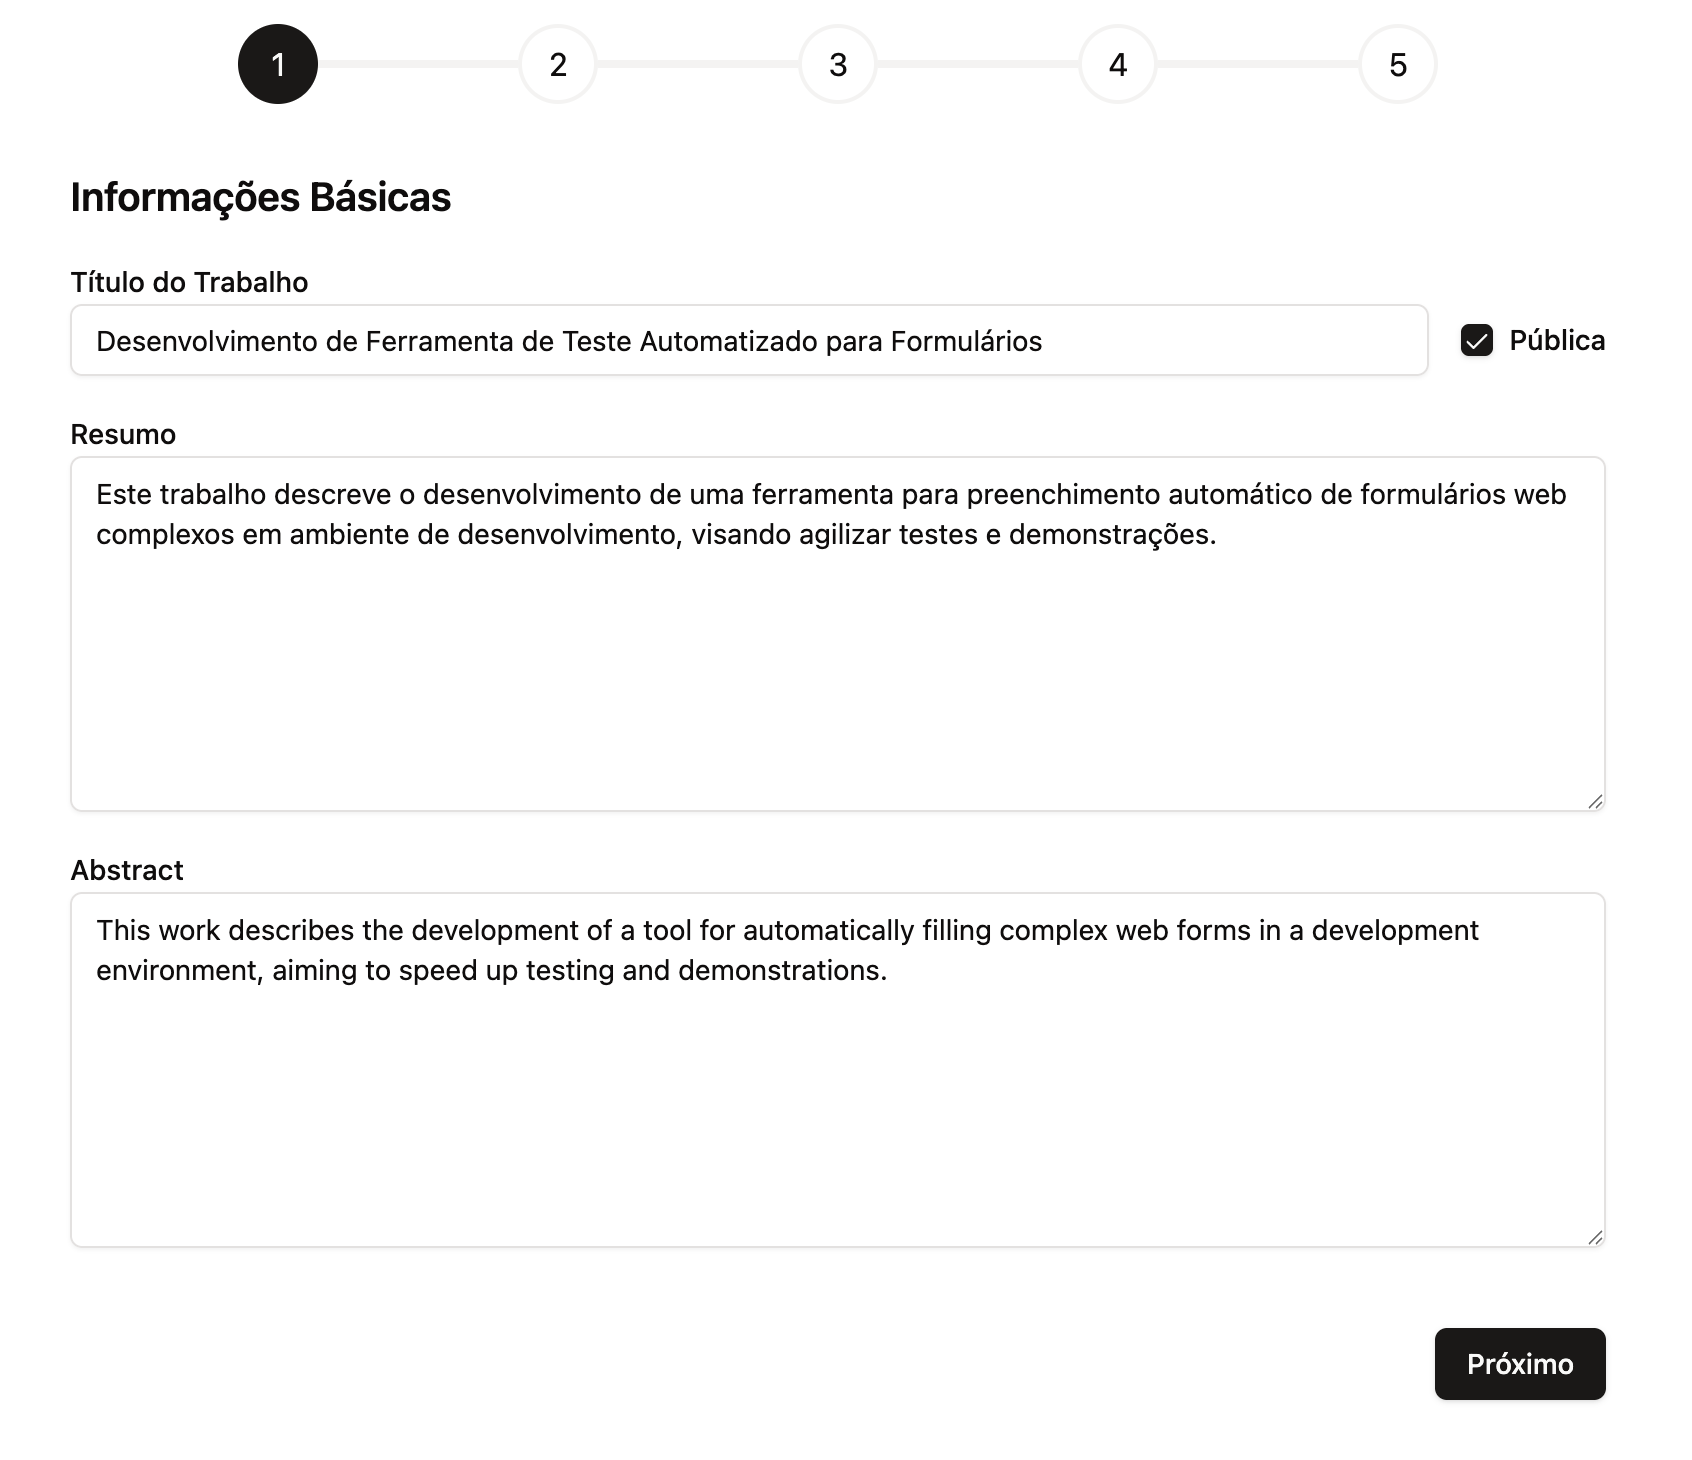
\includegraphics[width=0.9\textwidth]{multi-step-criacao-de-banca-1.png}
    \end{center}
    \vspace{0.3em}
    \small
    Primeira etapa: título, resumo, abstract e controle de visibilidade pública
\end{frame}

\begin{frame}{Multi-Step Wizard: Etapa 2 - Informações do Autor}
    \begin{center}
        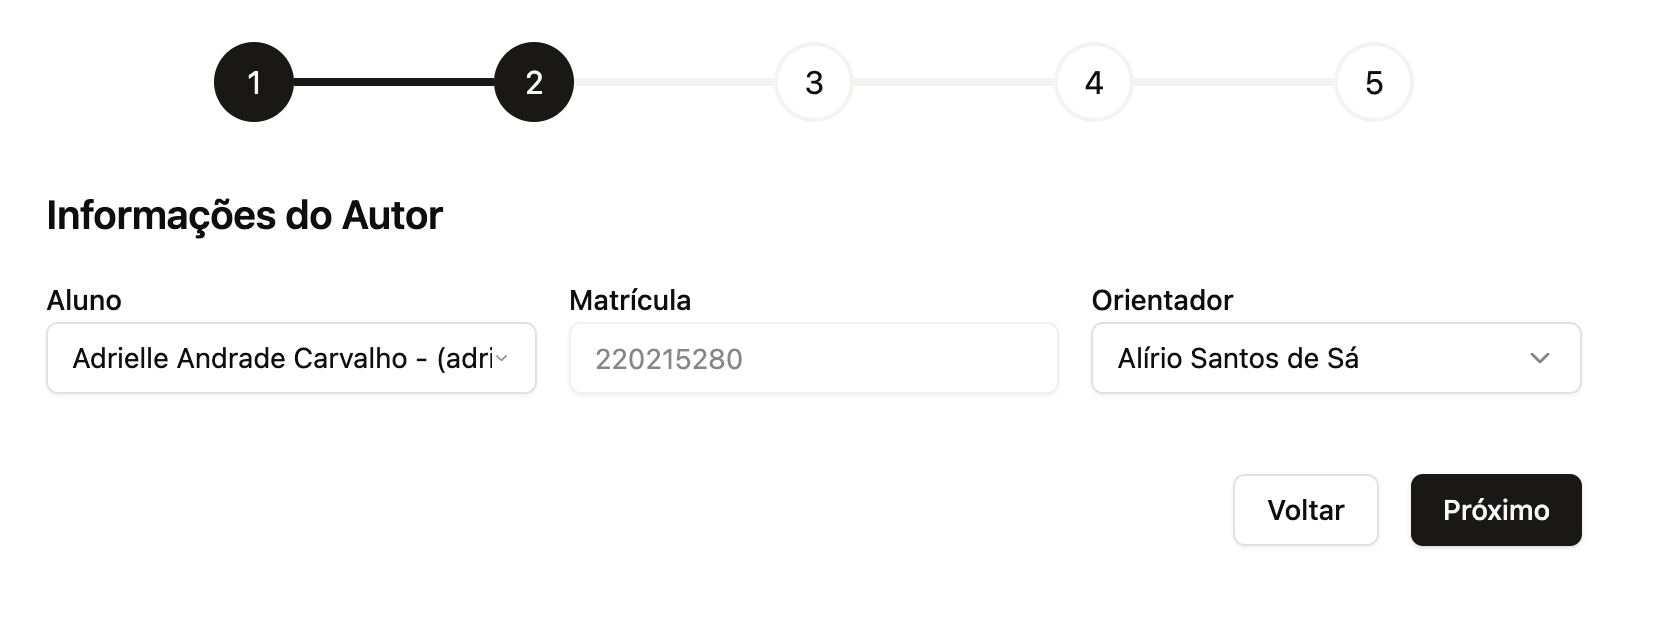
\includegraphics[width=0.9\textwidth]{multi-step-criacao-de-banca-2.png}
    \end{center}
    \vspace{0.3em}
    \small
    Segunda etapa: dados do discente e seleção de orientador e coorientador
\end{frame}

\begin{frame}{Multi-Step Wizard: Etapa 3 - Avaliadores}
    \begin{center}
        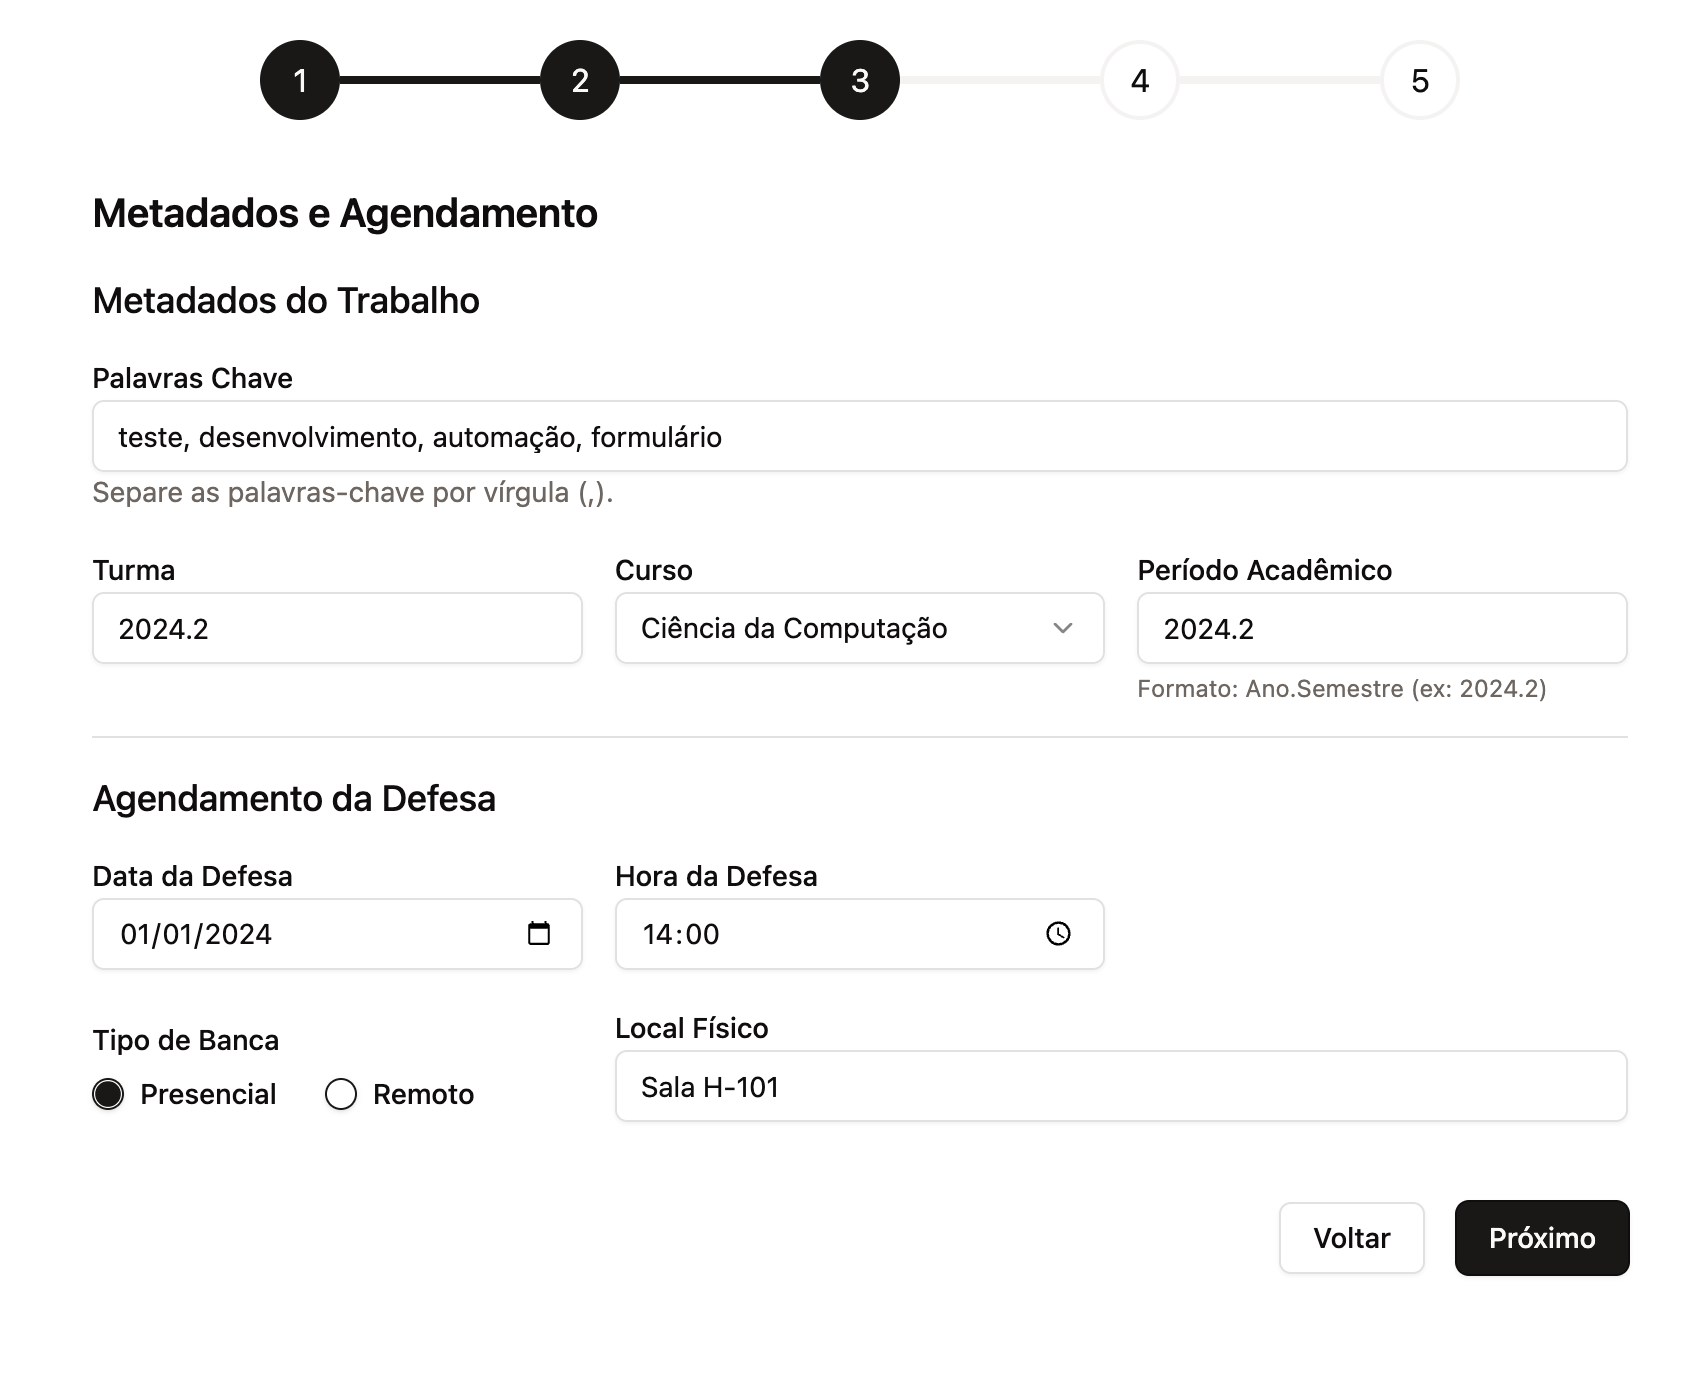
\includegraphics[width=0.9\textwidth]{multi-step-criacao-de-banca-3.png}
    \end{center}
    \vspace{0.3em}
    \small
    Terceira etapa: seleção de avaliadores internos e externos
\end{frame}

\begin{frame}{Multi-Step Wizard: Etapa 4 - Metadados Acadêmicos}
    \begin{center}
        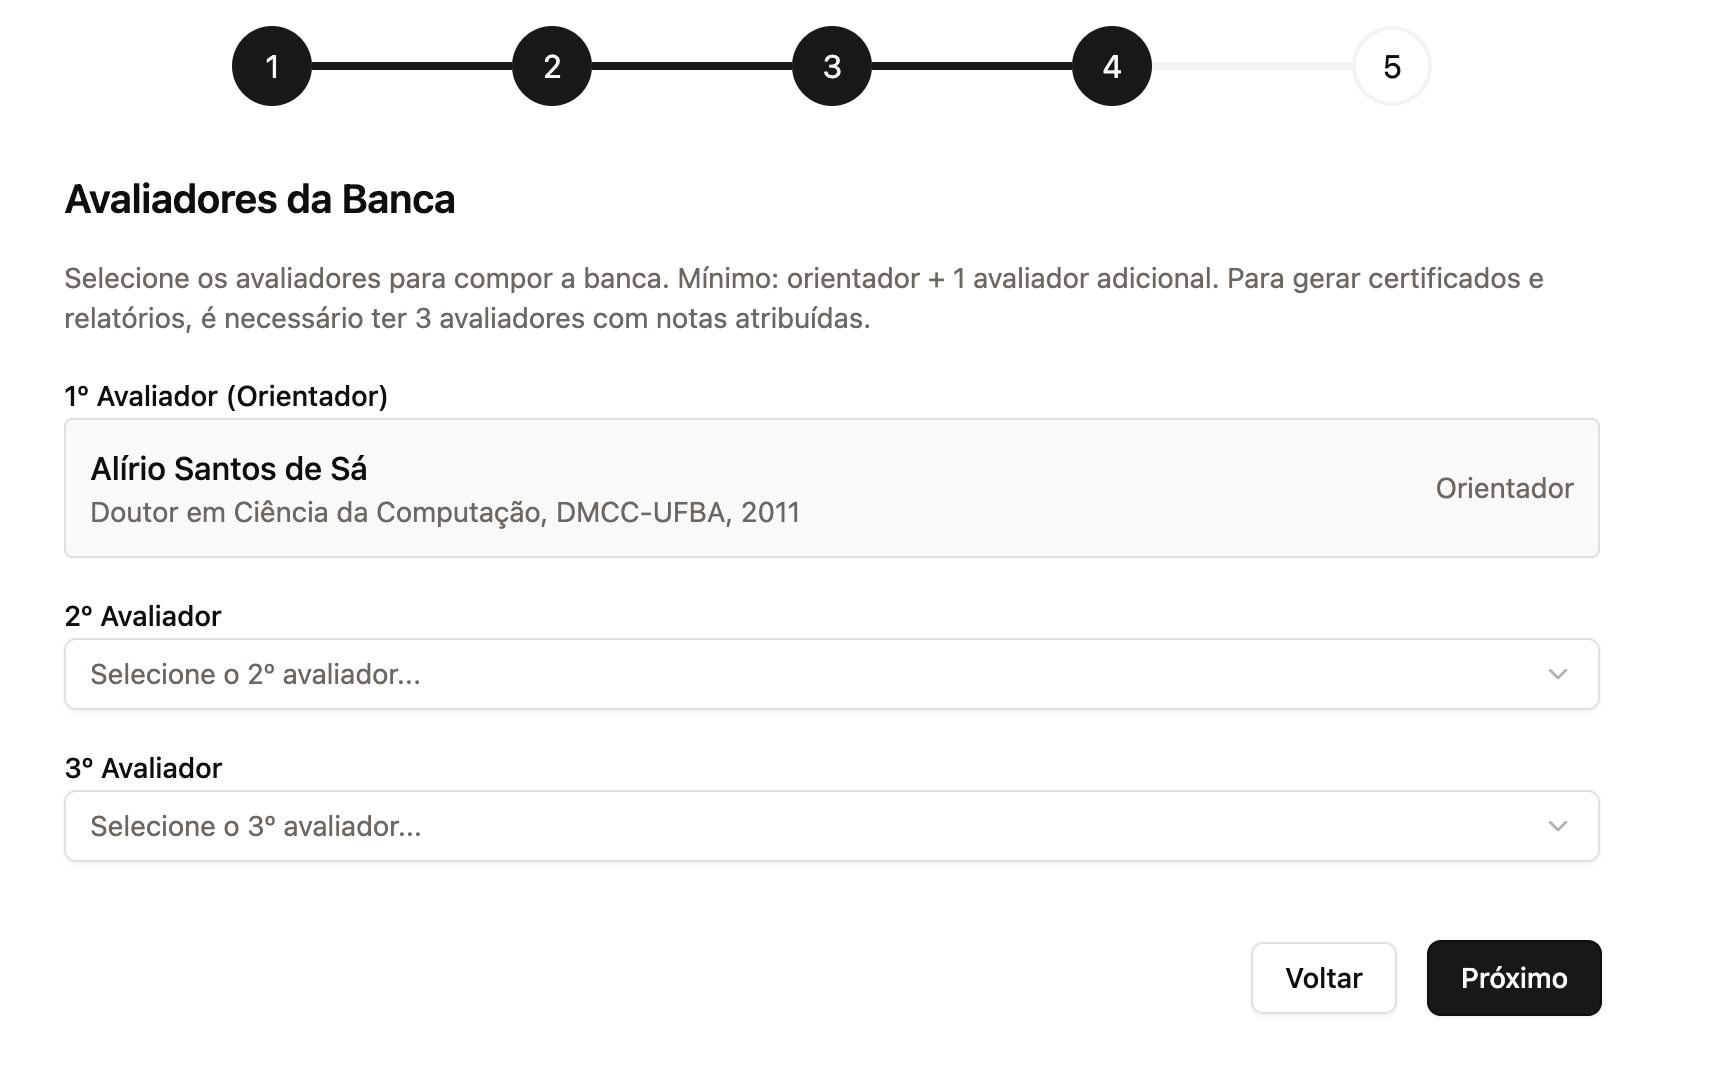
\includegraphics[width=0.9\textwidth]{multi-step-criacao-de-banca-4.png}
    \end{center}
    \vspace{0.3em}
    \small
    Quarta etapa: curso, tipo de trabalho, palavras-chave e área de concentração
\end{frame}

\begin{frame}{Multi-Step Wizard: Etapa 5 - Revisão e Confirmação}
    \begin{center}
        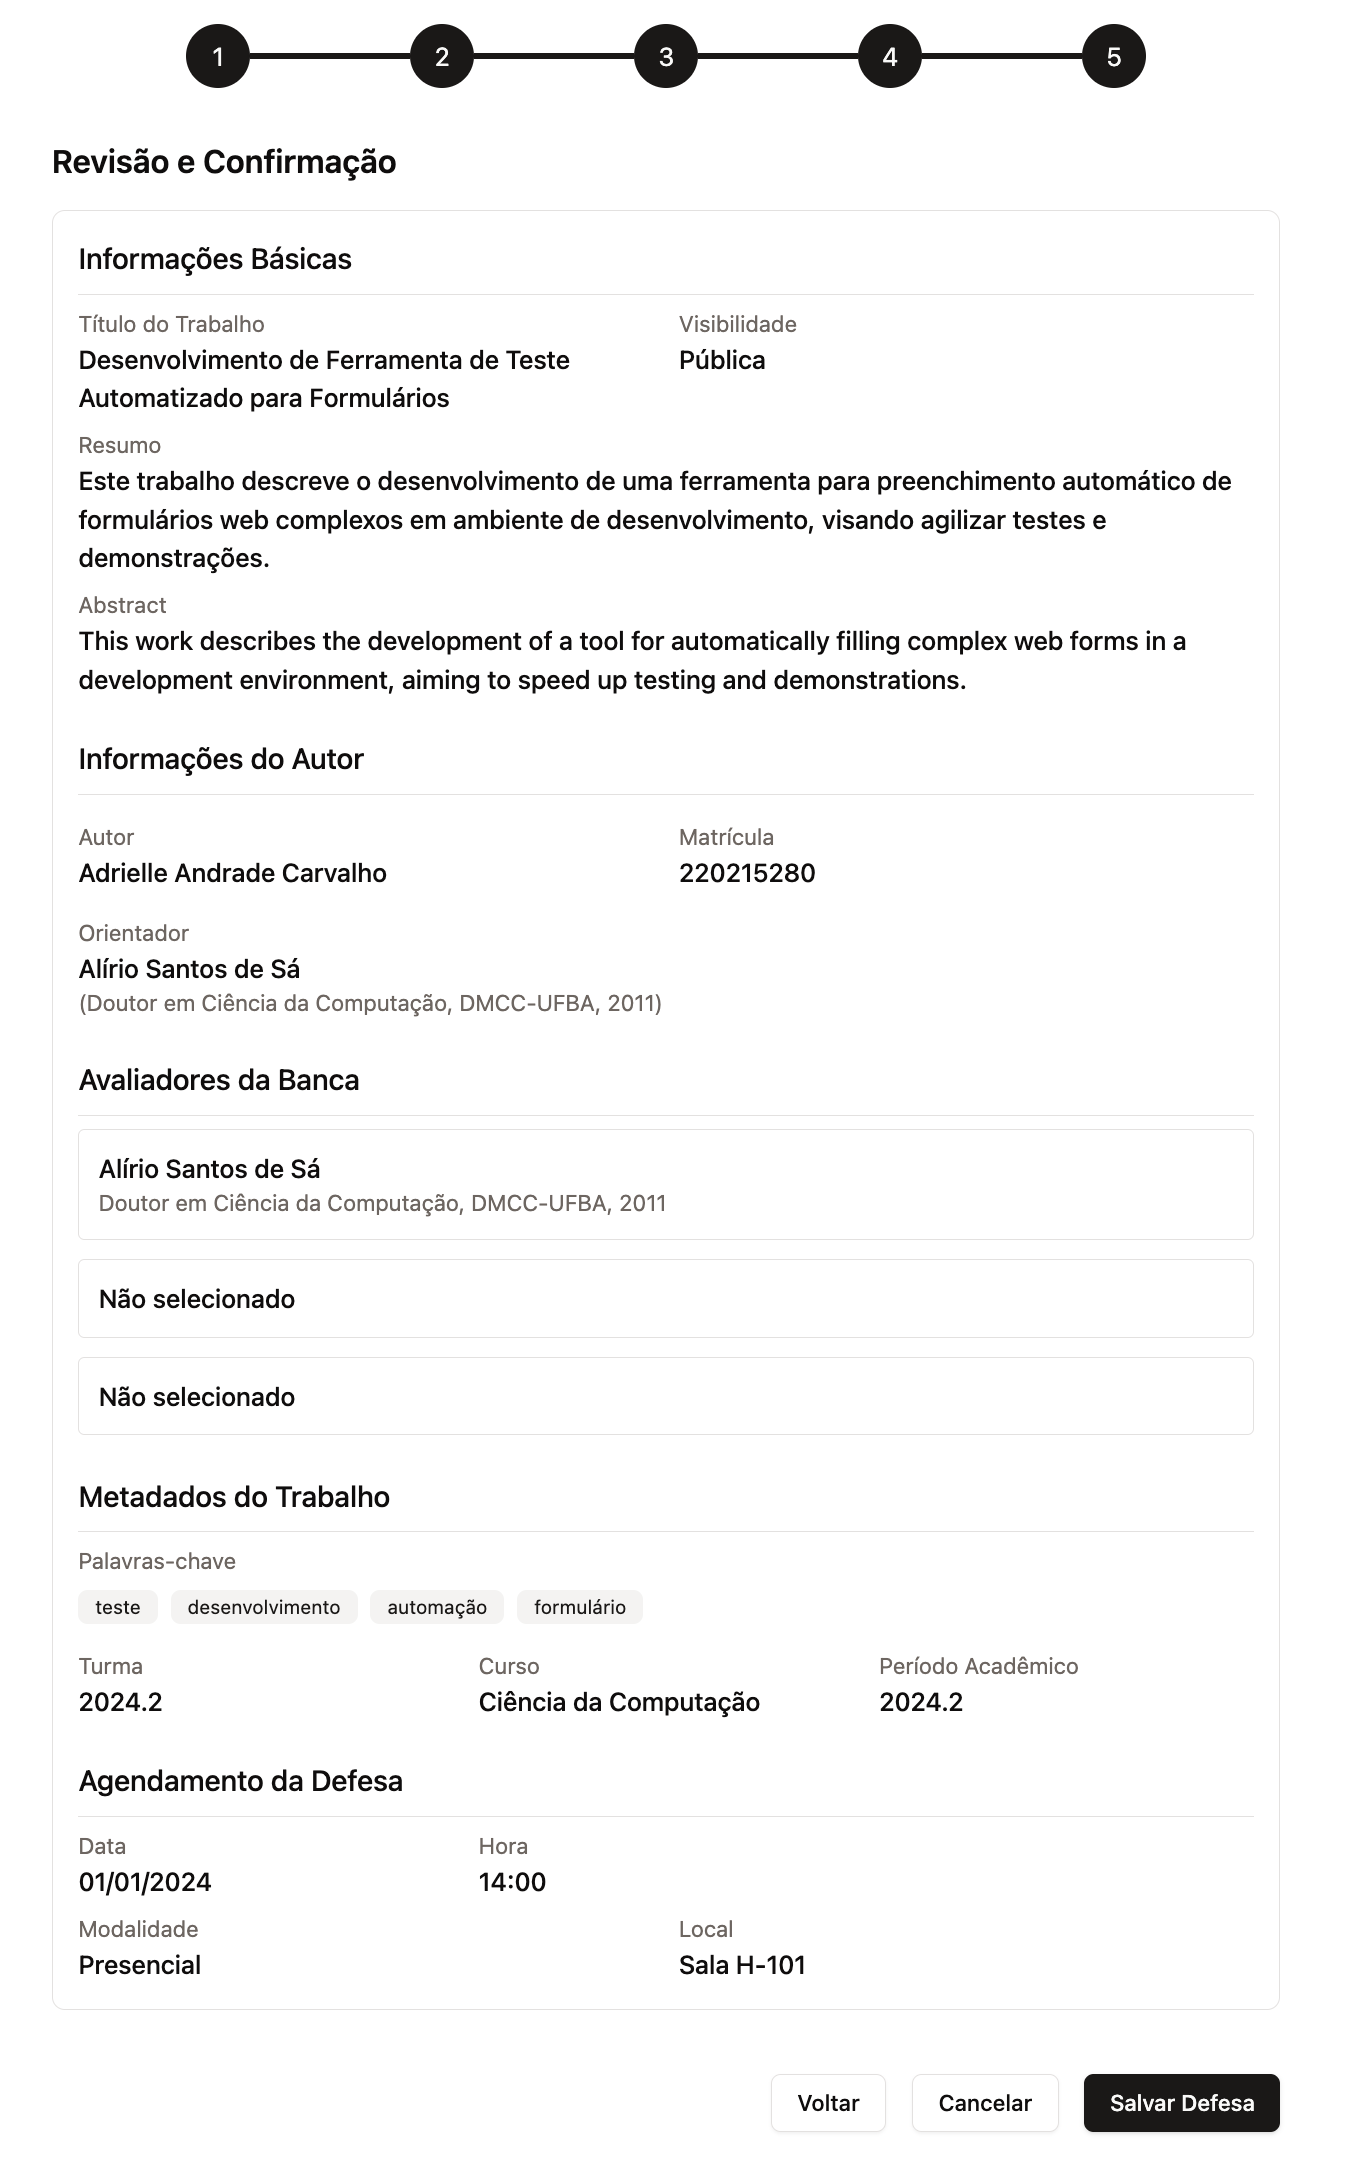
\includegraphics[width=0.9\textwidth]{multi-step-criacao-de-banca-resumo.png}
    \end{center}
    \vspace{0.3em}
    \small
    Quinta etapa: sumário consolidado de todas as informações antes da submissão
\end{frame}

\begin{frame}{Tela Inicial: Funcionalidades}
    \textbf{Interface Principal:}
    \begin{itemize}
        \item Organização cronológica automática:
        \begin{itemize}
            \item \textbf{Próximas defesas} (ordem ascendente)
            \item \textbf{Defesas anteriores} (ordem descendente)
        \end{itemize}
    \end{itemize}
    
    \vspace{0.5em}
    \textbf{Funcionalidades de Busca:}
    \begin{itemize}
        \item Filtro por múltiplos critérios (título, discente, orientador, avaliador)
        \item Paginação configurável (10/25/50 itens)
        \item Ordenação por múltiplas colunas
    \end{itemize}
    
    \vspace{0.5em}
    \textbf{Melhoria vs SISDEF 2.0:}
    \begin{itemize}
        \item Busca expandida (antes: só por título)
        \item Performance superior (paginação eficiente)
    \end{itemize}
\end{frame}

\begin{frame}{Tela Inicial e Visualização de Defesas}
    \begin{center}
        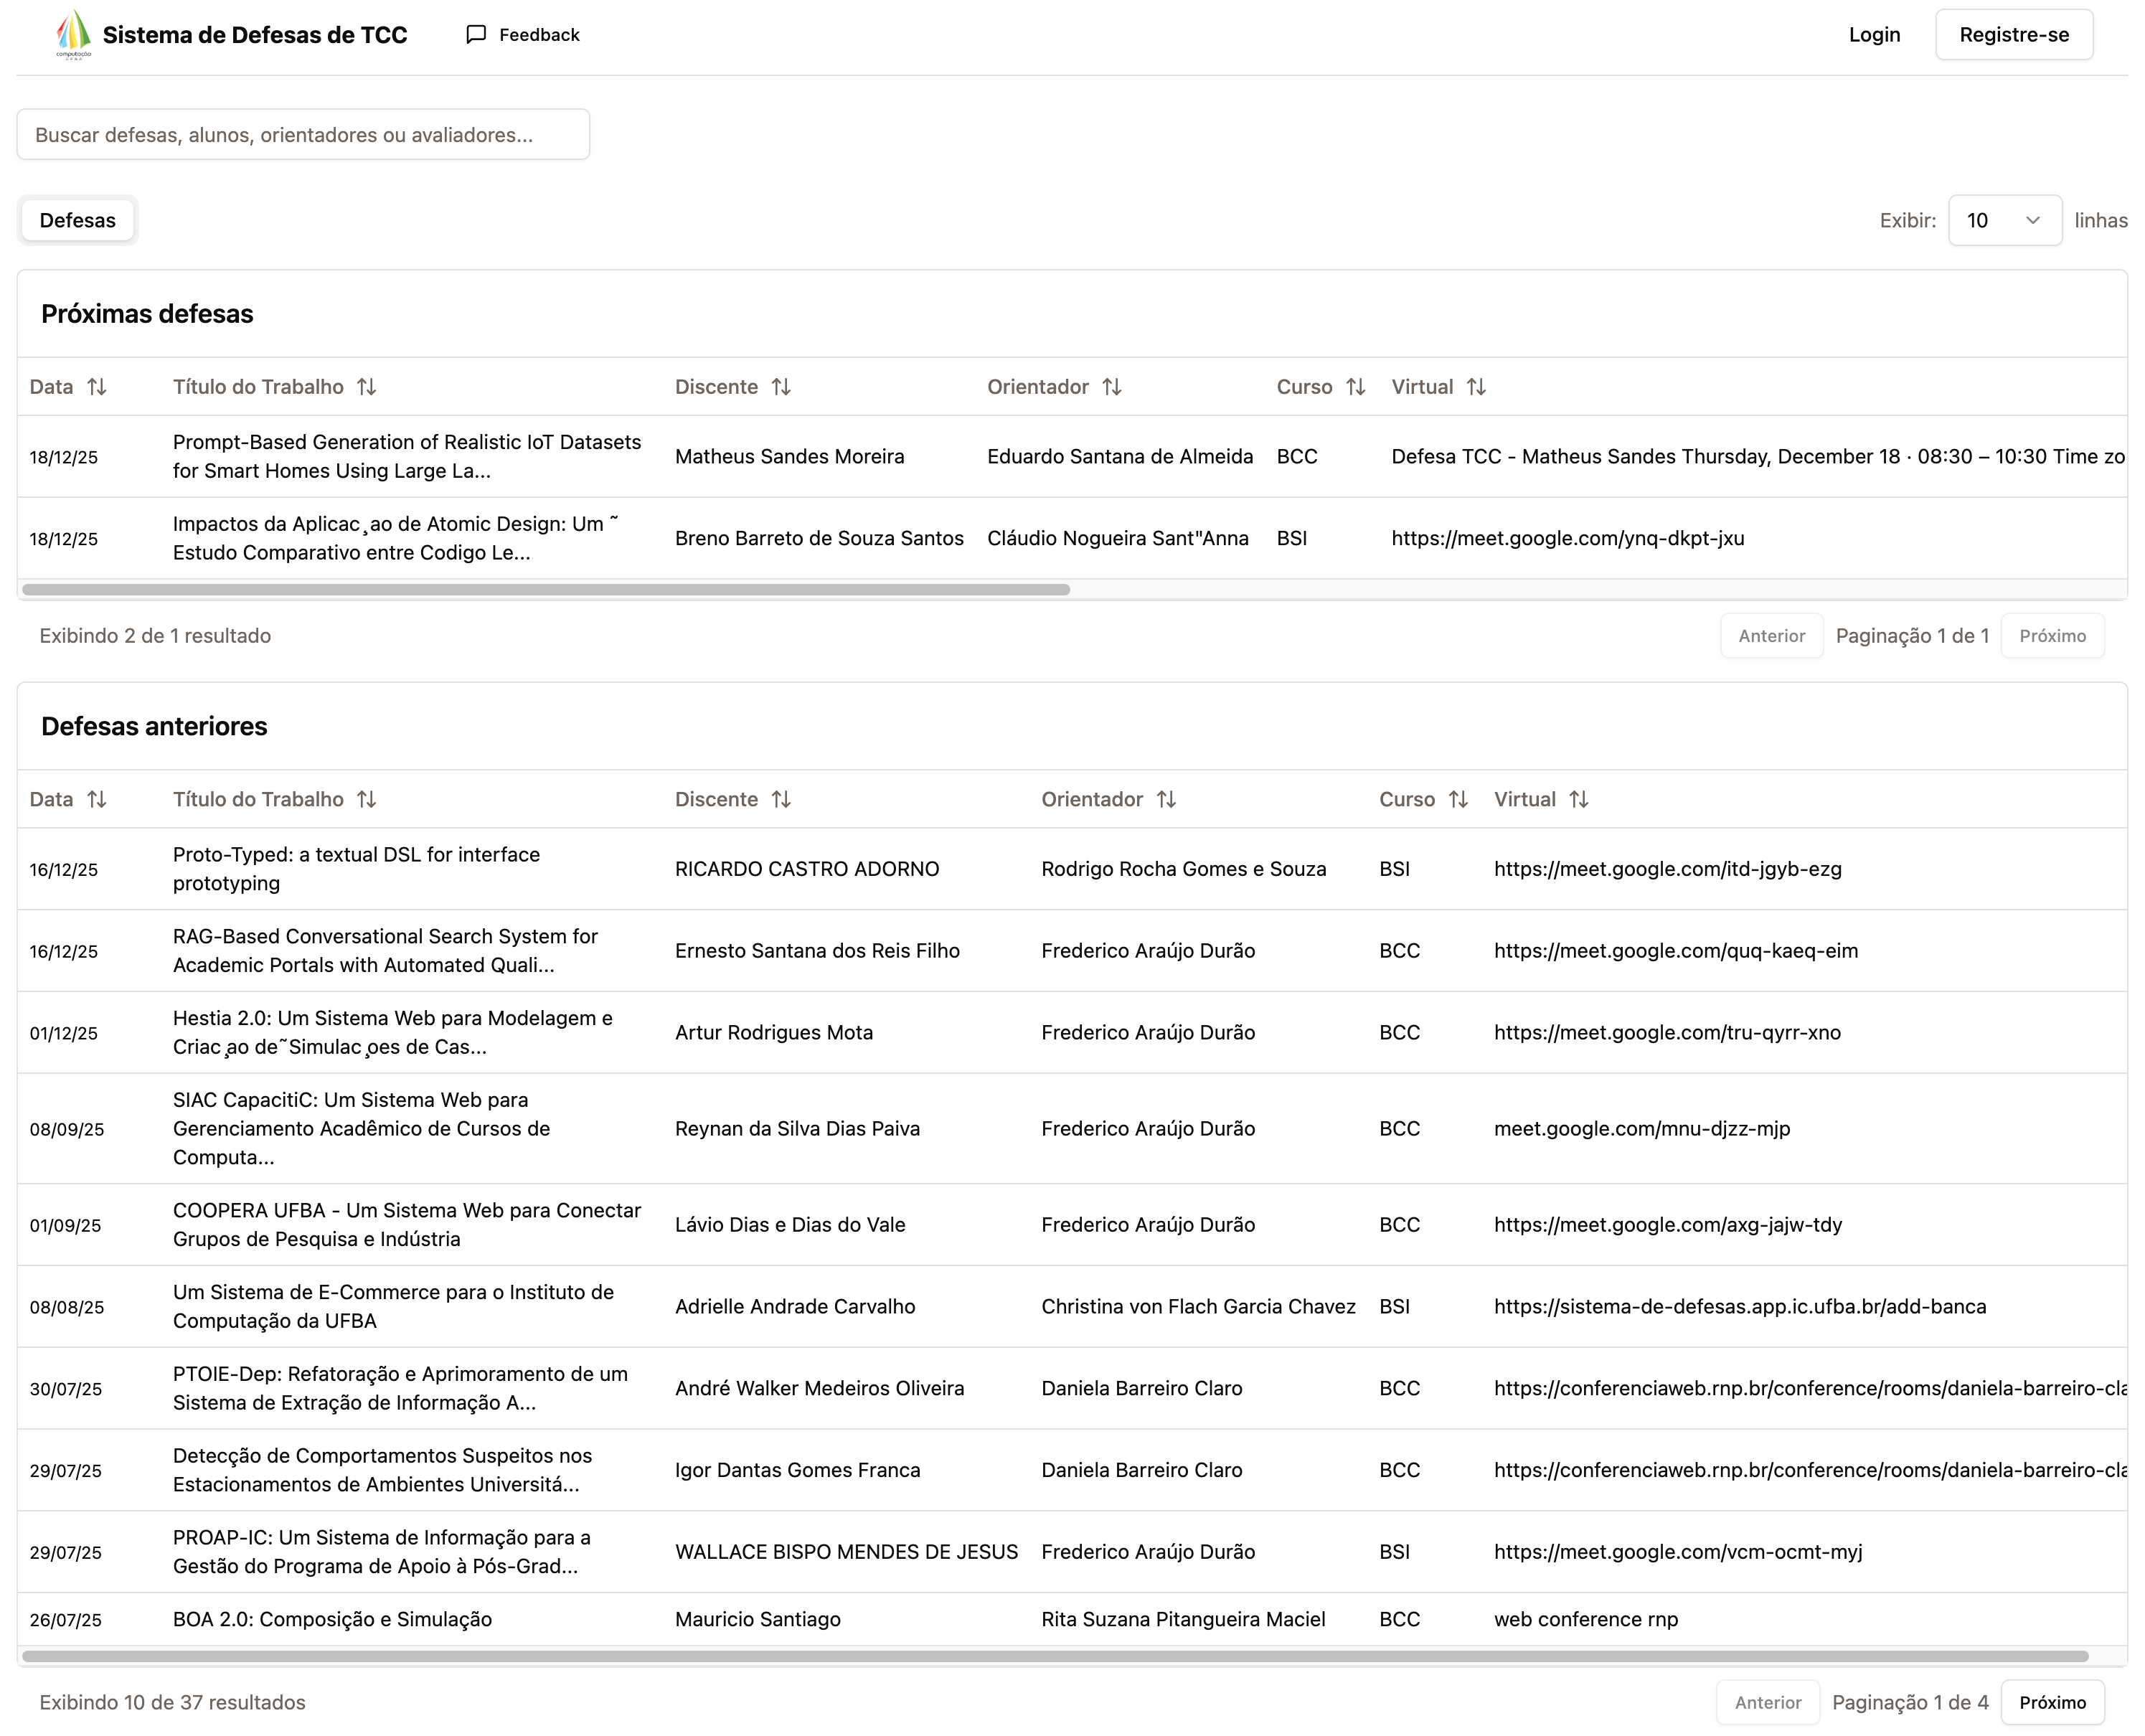
\includegraphics[width=0.95\textwidth]{tela-inicial-com-bancas-passadas-e-bancas-futuras.png}
    \end{center}
\end{frame}


\begin{frame}{Gerenciamento Administrativo de Usuários}
    \begin{center}
        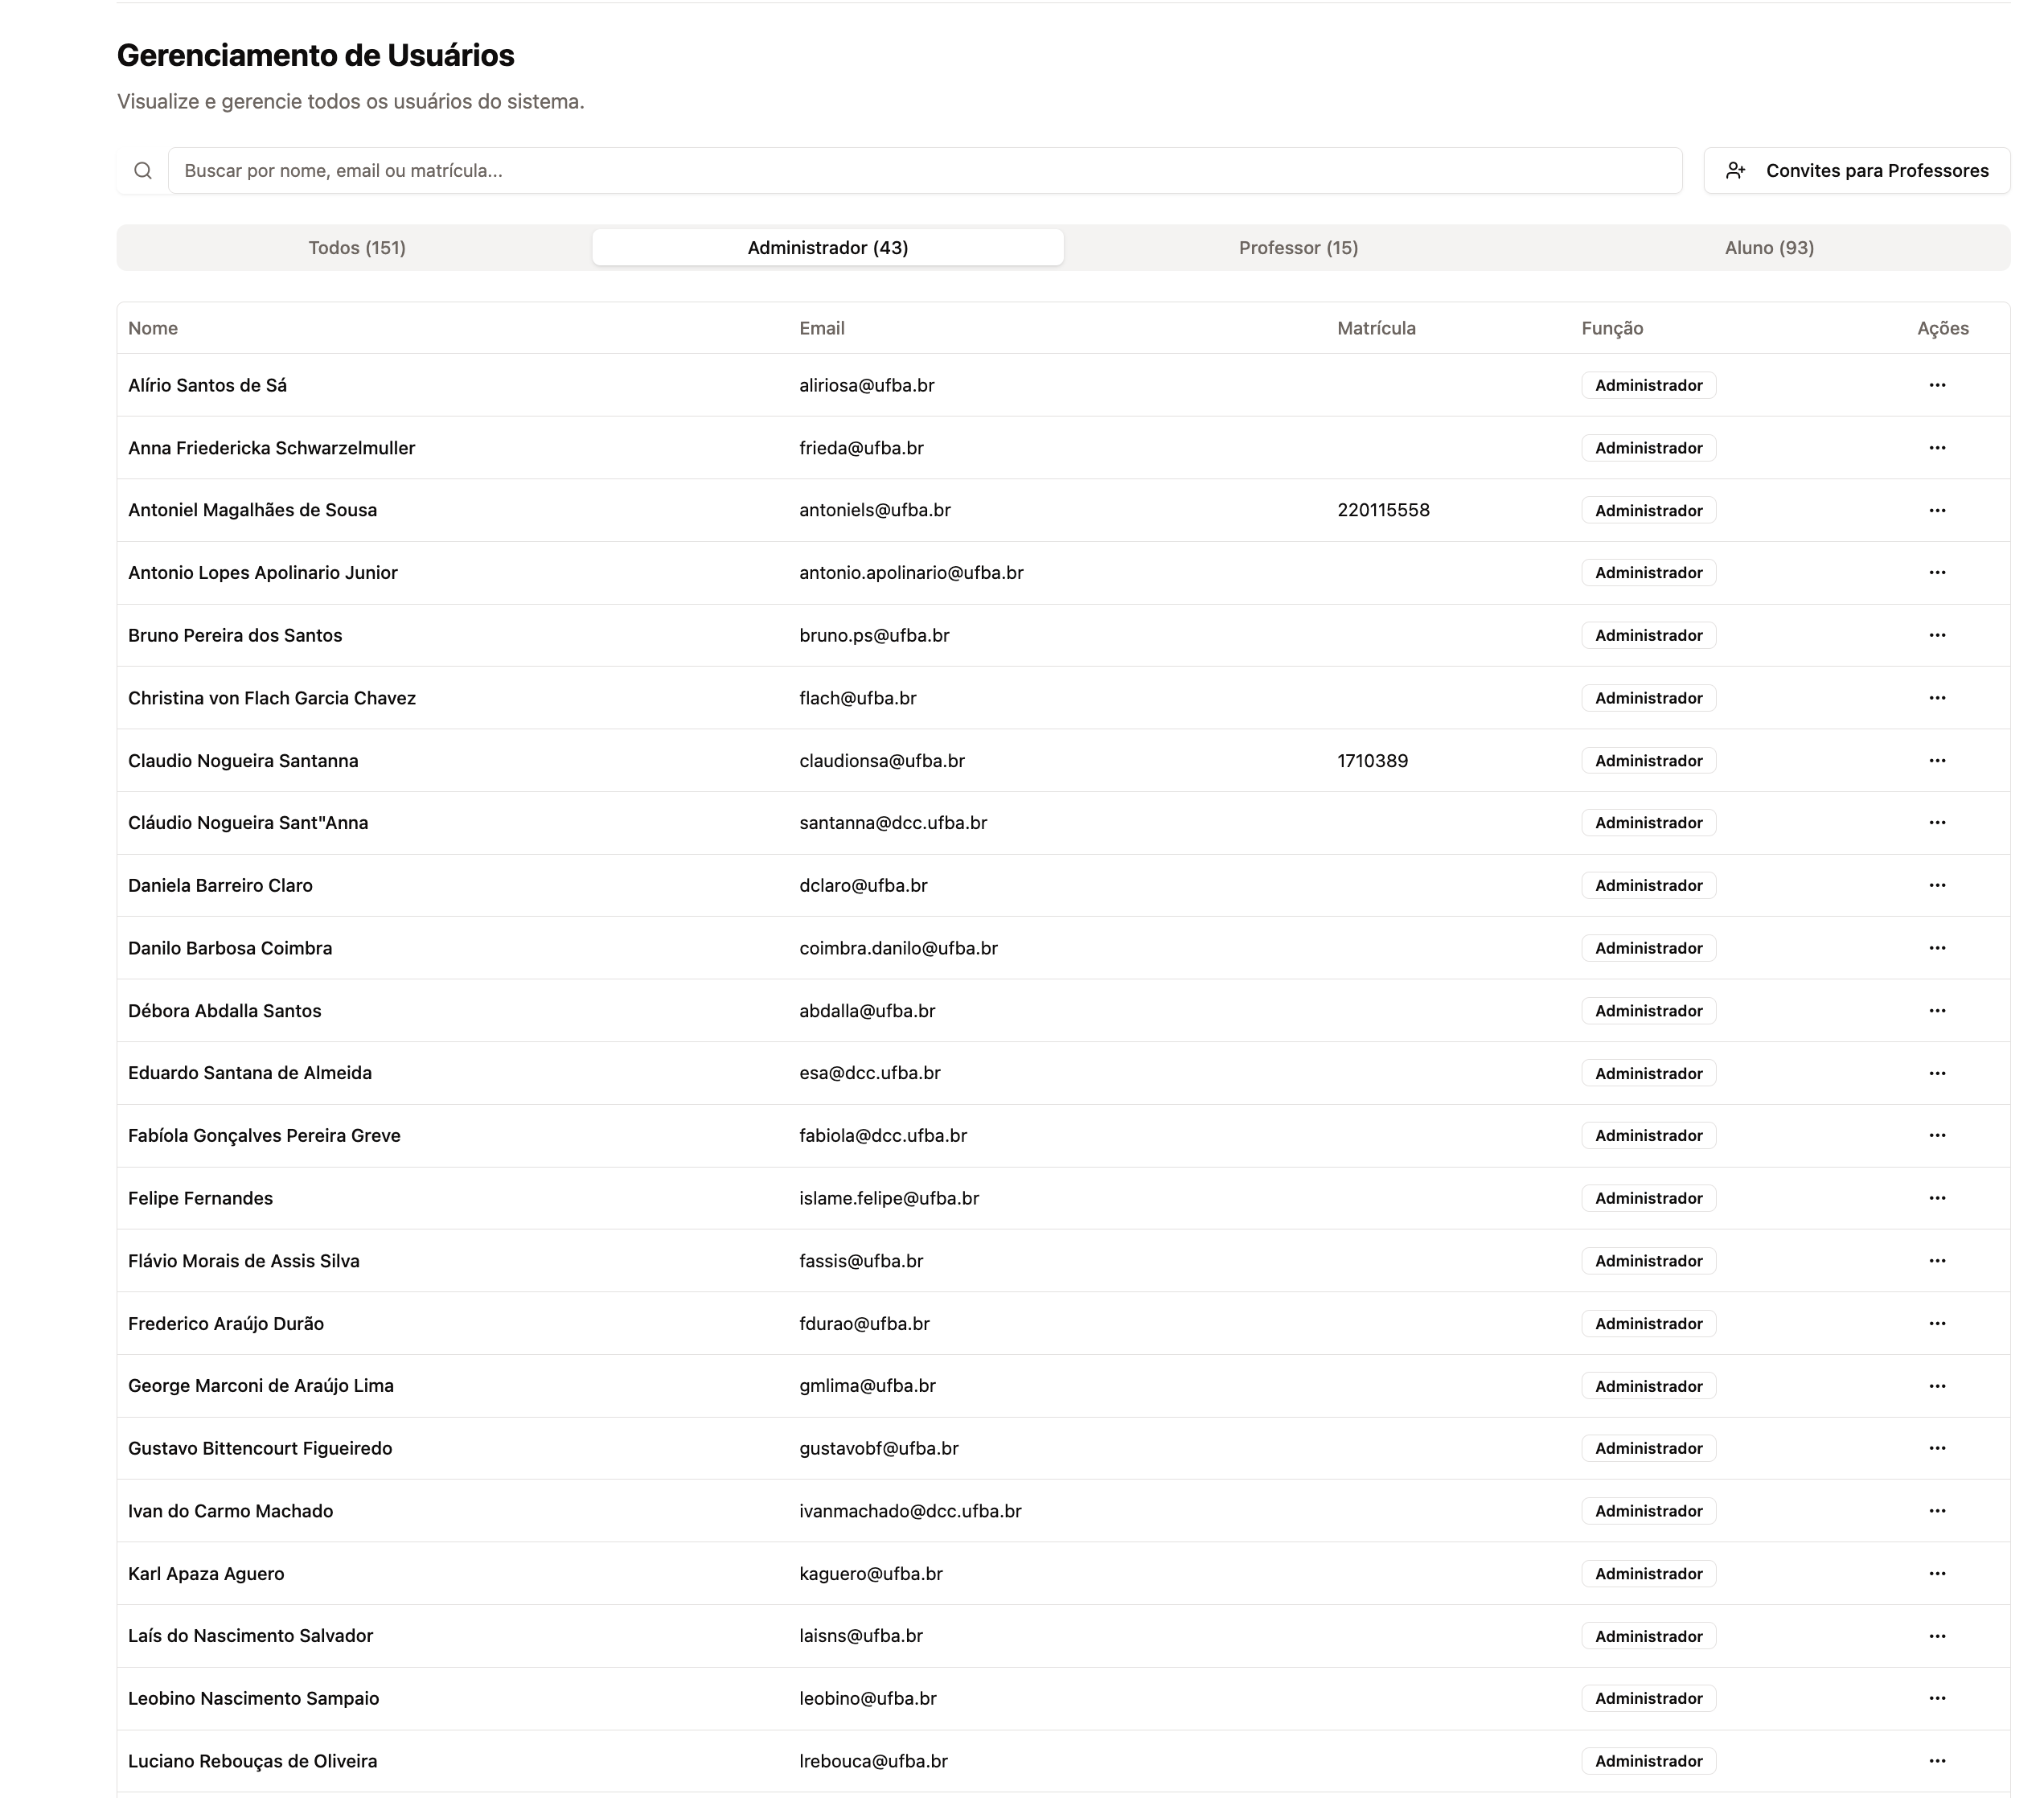
\includegraphics[width=0.95\textwidth]{gerenciamento-de-usuarios.png}
    \end{center}
\end{frame}
\begin{frame}{Gerenciamento de Usuários: Funcionalidades}
    \textbf{Painel de Usuários:}
    \begin{itemize}
        \item Visualização consolidada
        \item Filtros dinâmicos por perfil (tabs)
        \item Busca por nome/email/matrícula
        \item Ações administrativas (alteração de permissões, reset de senha)
    \end{itemize}
    
    \vspace{0.5em}
    \textbf{Convite de Professores Externos (Inovação):}
    \begin{itemize}
        \item Geração de links únicos de convite
        \item Pré-preenchimento automático de dados
        \item Email com instruções de primeiro acesso
        \item \textbf{Impacto}: Formação rápida de bancas com externos
    \end{itemize}
\end{frame}


\begin{frame}{Geração de Documentos PDF}
    \textbf{3 Tipos de Documentos (baseados em templates oficiais UFBA):}
    \begin{enumerate}
        \item \textbf{Formulário de Avaliação}
        \begin{itemize}
            \item Para registro de notas por cada avaliador
            \item Pré-preenchido com dados da banca
        \end{itemize}
        \item \textbf{Declaração de Participação}
        \begin{itemize}
            \item Para membros da banca
            \item Comprovação de atuação como avaliador
        \end{itemize}
        \item \textbf{Declaração de Orientação}
        \begin{itemize}
            \item Para orientadores
            \item Comprovação de orientação do trabalho
        \end{itemize}
    \end{enumerate}
    
    \textbf{Impacto:}
    \begin{itemize}
        \item Elimina tarefa altamente repetitiva
        \item Reduz erros humanos no preenchimento
        \item Economiza tempo de docentes
    \end{itemize}
\end{frame}

\begin{frame}{Detalhamento de Informações de Banca}
    \begin{center}
        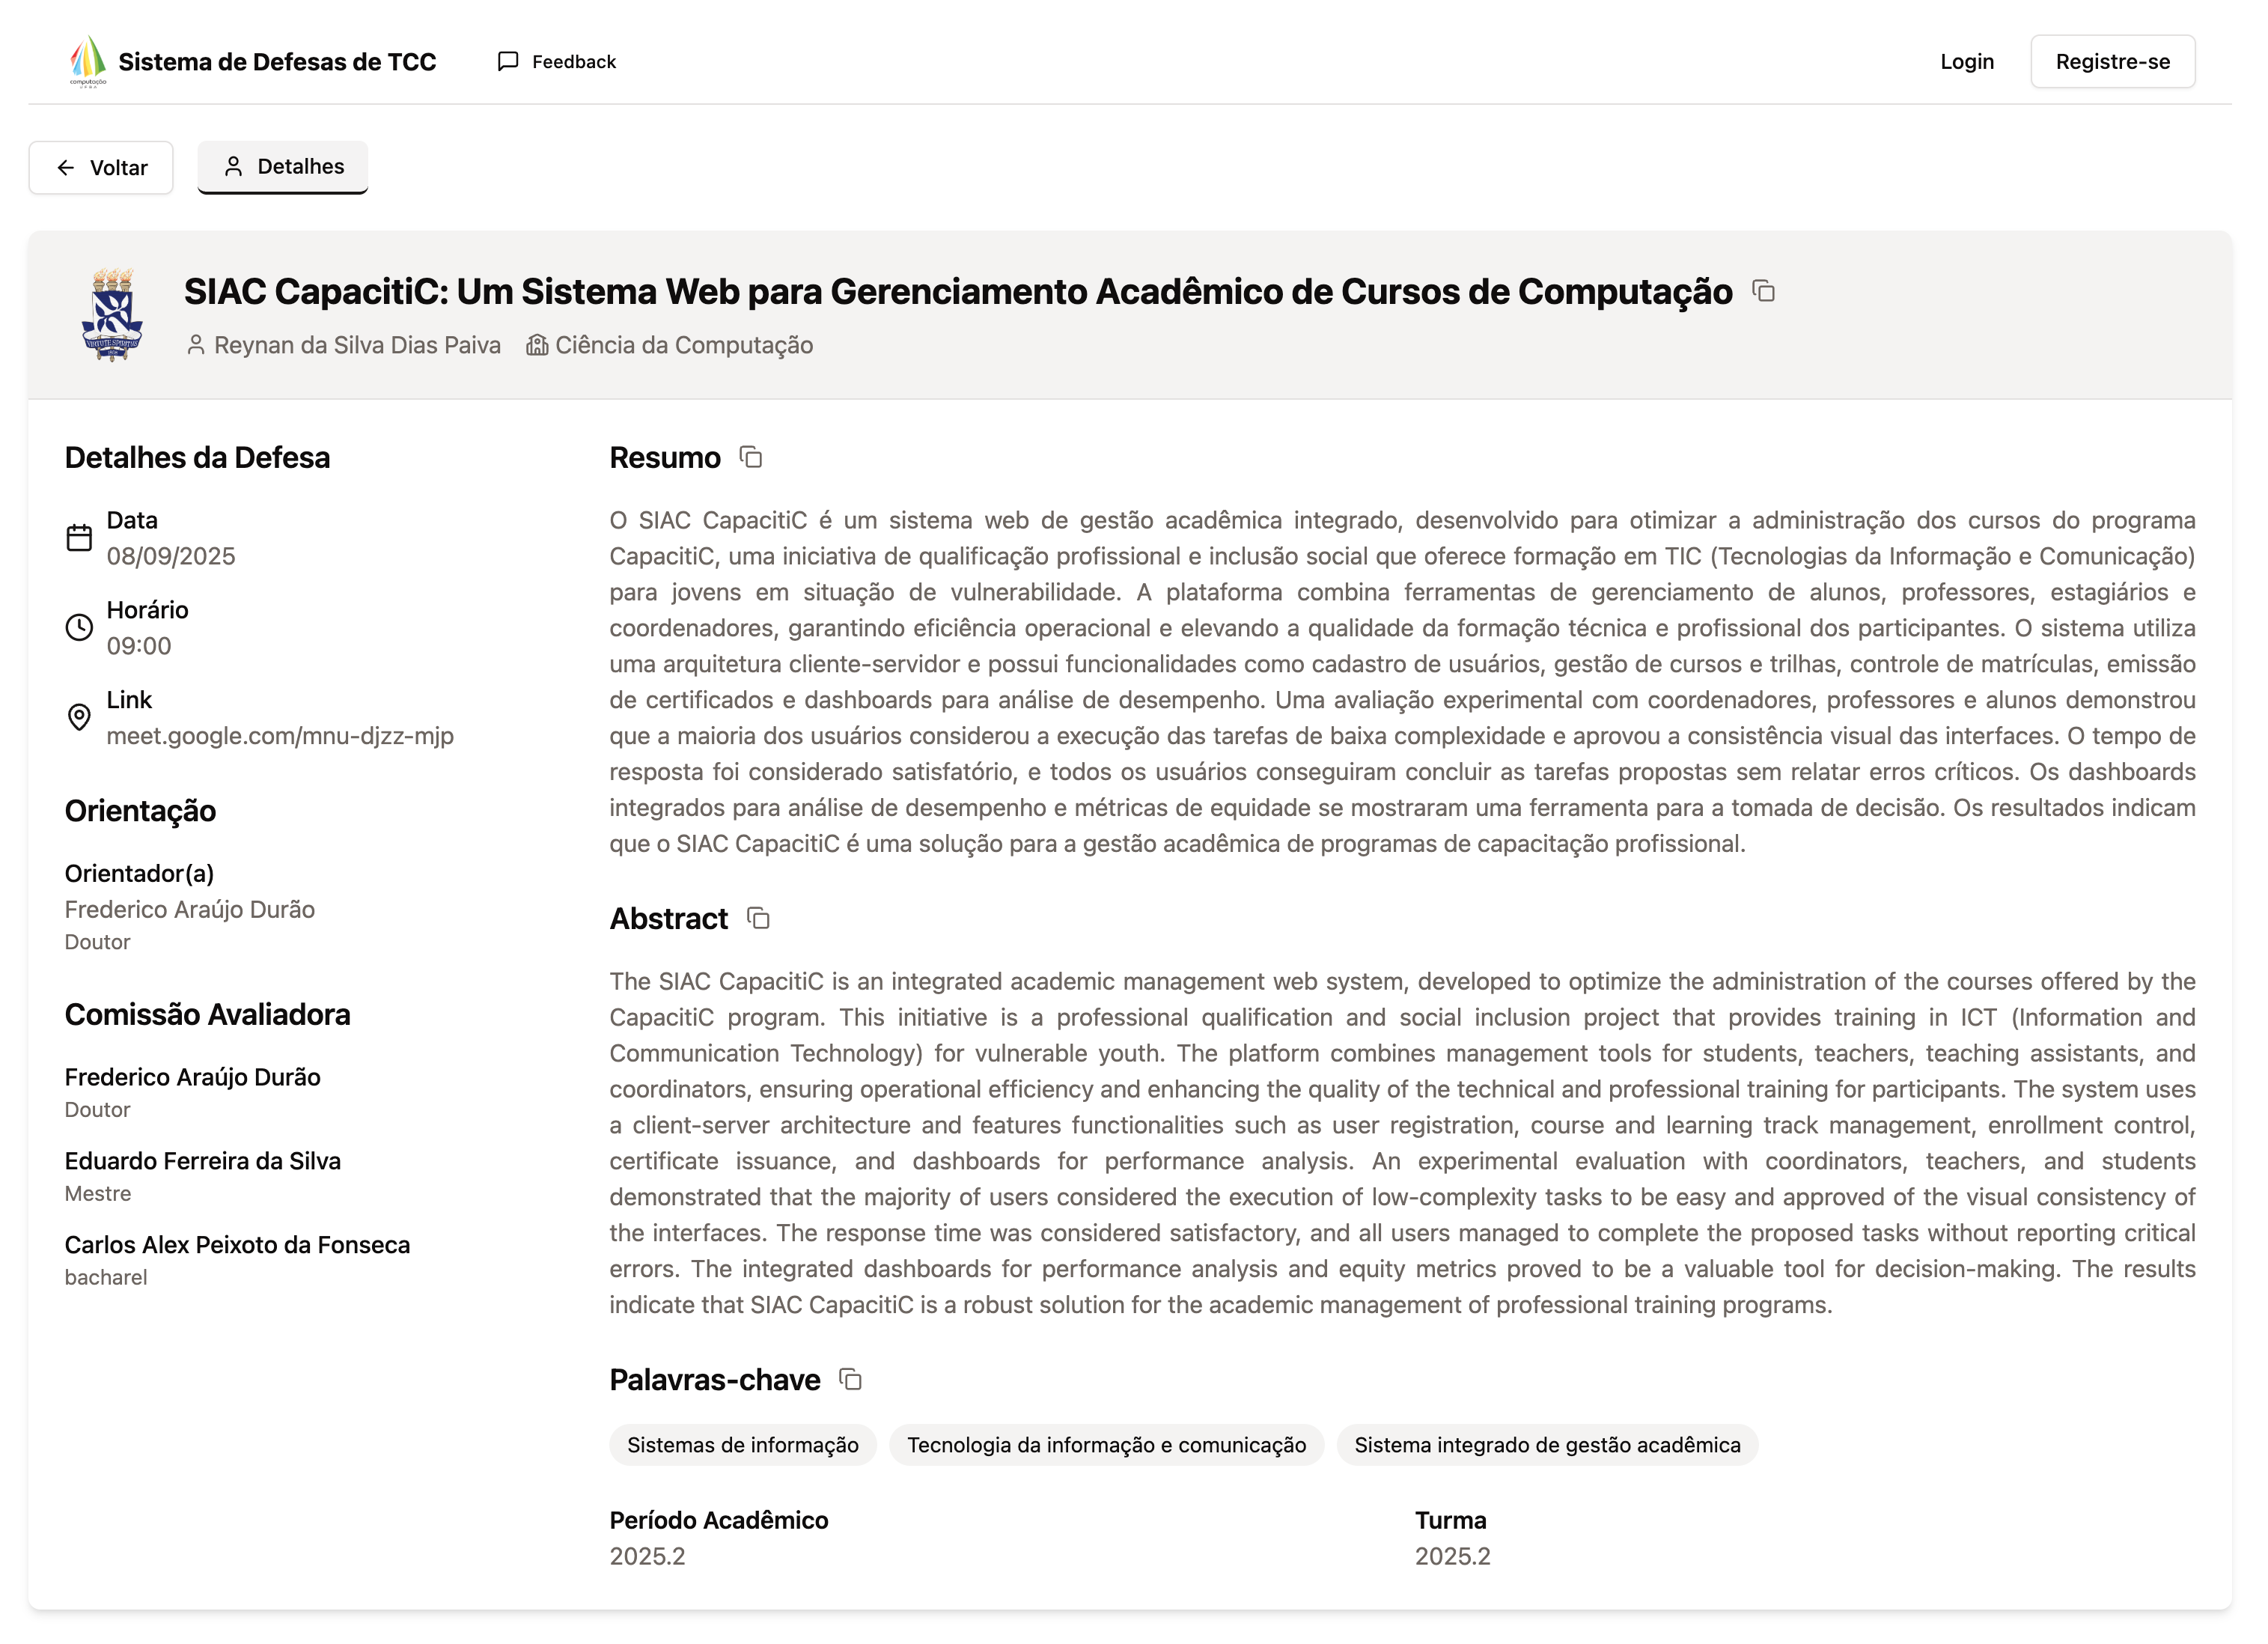
\includegraphics[width=0.95\textwidth]{tela-de-com-informacao-de-bancas.png}
    \end{center}
\end{frame}

\begin{frame}{Detalhes de Banca: Funcionalidades}
    \textbf{Tela Consolidada:}
    \begin{itemize}
        \item Agrupamento lógico de informações:
        \begin{itemize}
            \item Dados básicos do trabalho (título, resumo, abstract)
            \item Informações do autor (nome, matrícula)
            \item Composição da banca (orientador, coorientador, avaliadores)
            \item Metadados acadêmicos (curso, tipo, palavras-chave)
            \item Agendamento (data, horário, local, link virtual)
        \end{itemize}
    \end{itemize}
    
    \vspace{0.5em}
    \textbf{Ações Contextuais (para usuários autorizados):}
    \begin{itemize}
        \item Edição de informações
        \item Geração de documentos
        \item Gerenciamento de notas dos avaliadores
    \end{itemize}
\end{frame}

\begin{frame}{Perfil e Configurações Pessoais}
    \begin{center}
        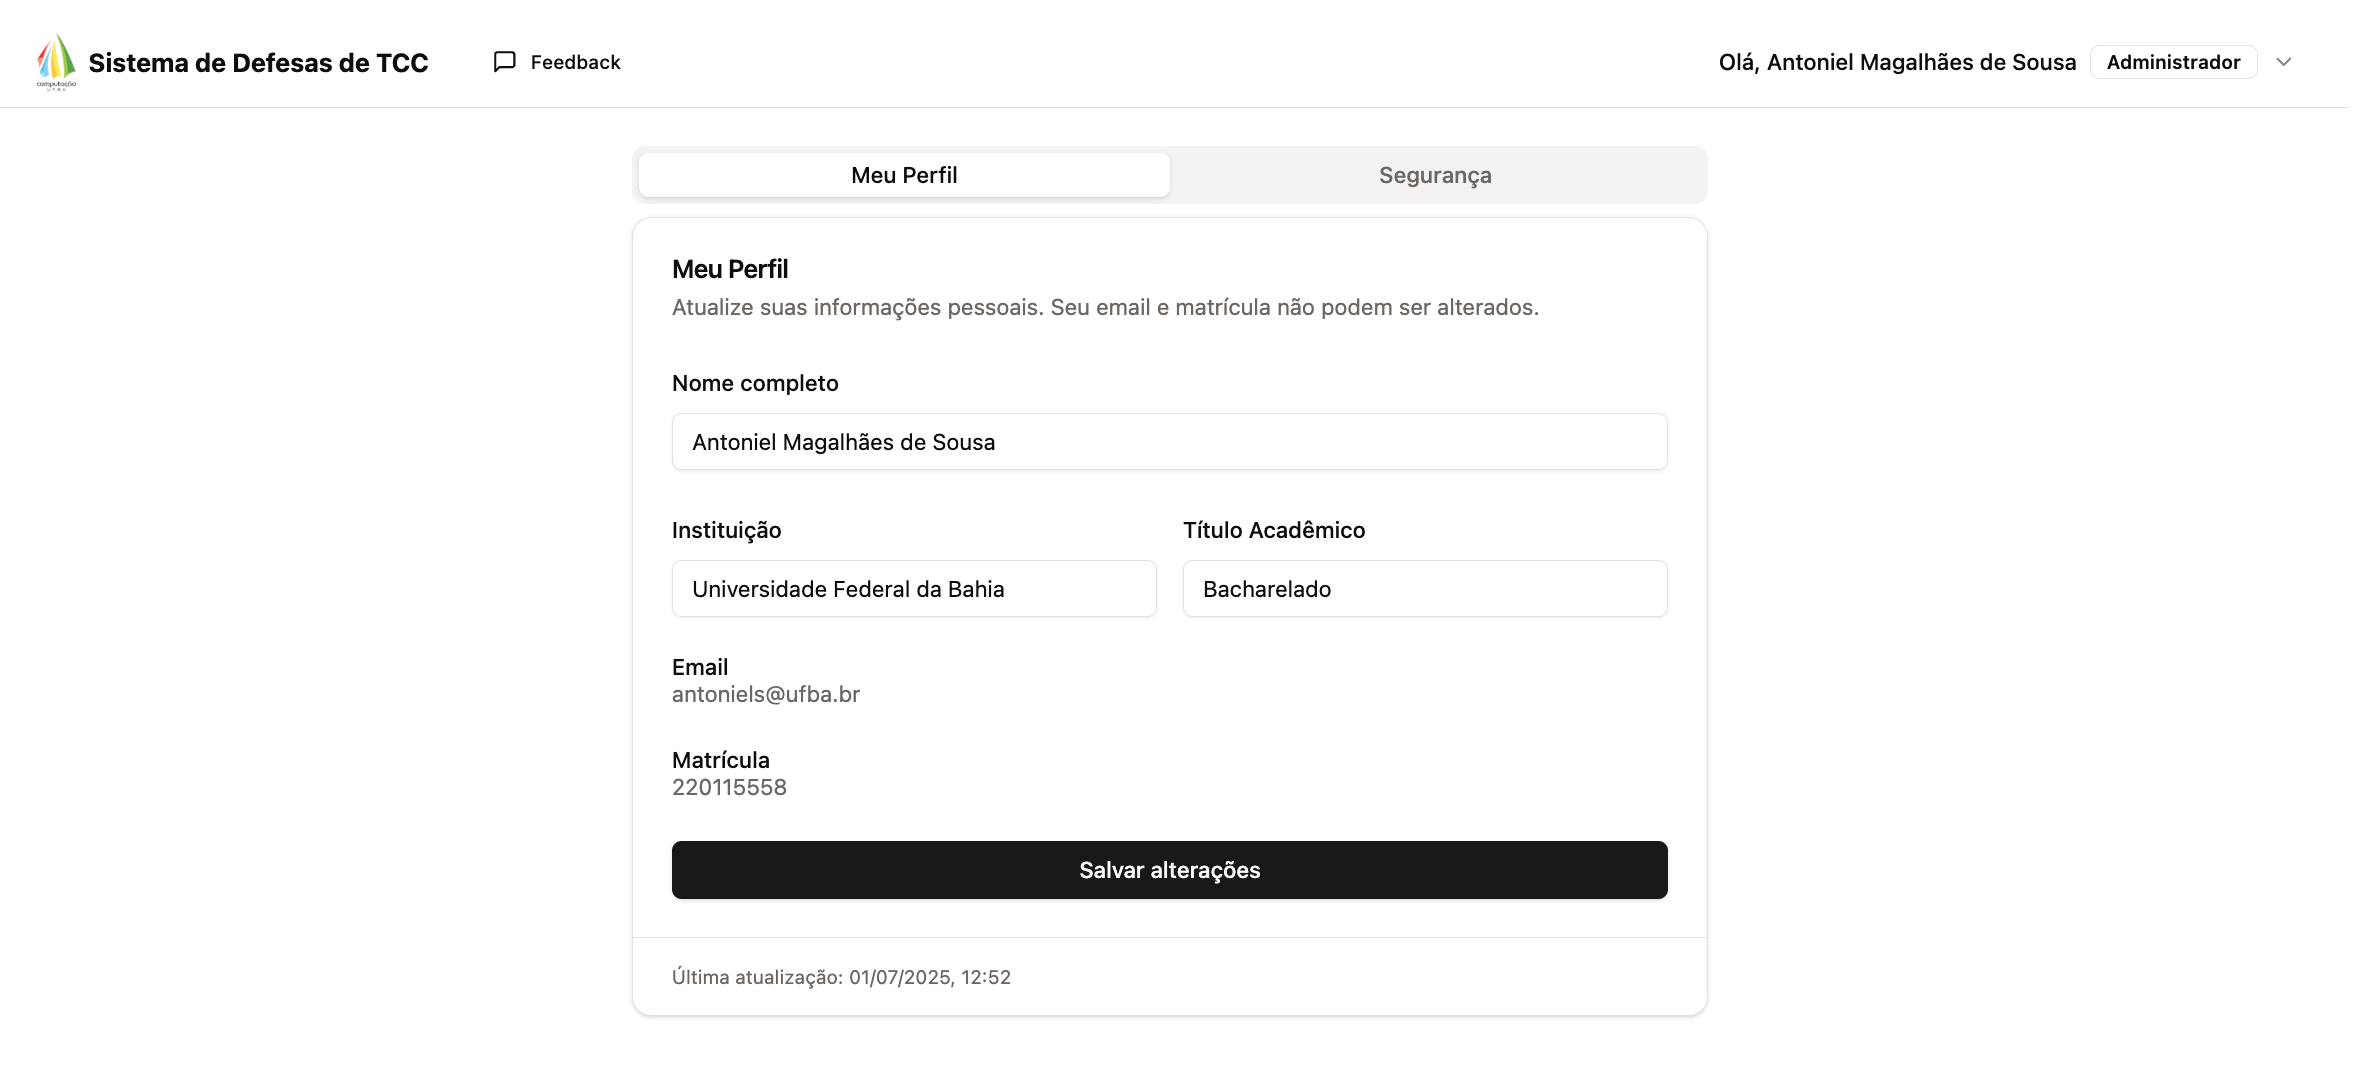
\includegraphics[width=0.95\textwidth]{tela-de-perfil-do-usuario.png}
    \end{center}
\end{frame}

%=================================================
\section{Arquitetura e Contribuições Técnicas}
%=================================================

\begin{frame}{Arquitetura Modular por Domínio}
    \small
    \textbf{Organização baseada em Domain-Driven Design:}
    
    \vspace{0.5em}
    \hspace{0.5em}
    \begin{columns}[T]
        \column{0.45\textwidth}
        \textbf{Módulos:}
        \begin{itemize}
            \item \texttt{auth/} - Autenticação e autorização
            \item \texttt{banca/} - Gerenciamento de bancas
            \item \texttt{usuario/} - Gerenciamento de usuários
            \item \texttt{curso/} - Gerenciamento de cursos
            \item \texttt{documento/} - Geração de documentos
        \end{itemize}
        
        \column{0.45\textwidth}
        \textbf{Cada módulo contém:}
        \begin{itemize}
            \item \texttt{*.route.ts} - Endpoints HTTP + validação
            \item \texttt{*.service.ts} - Lógica de negócio isolada
            \item \texttt{*.schema.ts} - Schemas Zod para validação
            \item \texttt{*.test.ts} - Testes unitários
        \end{itemize}
    \end{columns}
\end{frame}

\begin{frame}{Type Safety End-to-End}
    \textbf{Problema no SISDEF 2.0:}
    \begin{itemize}
        \item Erros de contrato entre frontend/backend só descobertos em runtime
        \item Mudanças no backend quebram frontend silenciosamente
        \item Debugging difícil e demorado
    \end{itemize}
\end{frame}

\begin{frame}{Type Safety End-to-End}
    \textbf{Solução - Hono RPC Client:}
    \begin{itemize}
        \item Backend define tipos explicitamente
        \item Frontend importa tipos automaticamente
        \item TypeScript valida contratos em \textbf{compile-time}
    \end{itemize}
    
    \vspace{0.5em}
    \textbf{Impactos:}
    \begin{itemize}
        \item  Contratos validados em compile-time
        \item  Autocompletar completo no frontend
        \item  Refatoração segura
        \item  \textbf{Elimina classe inteira de erros}
    \end{itemize}
\end{frame}

\begin{frame}{Suíte Completa de Testes}
    \textbf{Estado Anterior (SISDEF 1.0 e 2.0):}
    \begin{itemize}
        \item \textbf{Zero testes automatizados}
        \item Refatorações = arriscadas
        \item Regressões descobertas em produção
        \item Debugging manual e demorado
    \end{itemize}
\end{frame}

\begin{frame}{Suíte Completa de Testes}
    \textbf{Estratégia do SISDEF 3.0:}
    
    \begin{columns}[T]
        \column{0.45\textwidth}
        \textbf{Testes Unitários (Vitest):}
        \begin{itemize}
            \item Foco: Lógica de negócio isolada
            \item Execução rápida (JIT TypeScript)
            \item Watch mode inteligente
        \end{itemize}
        
        \column{0.45\textwidth}
        \textbf{Testes End-to-End (Playwright):}
        \begin{itemize}
            \item Foco: Fluxos críticos completos
            \item Múltiplos navegadores
            \item Banco de teste isolado (PGlite)
        \end{itemize}
    \end{columns}
    
    \vspace{0.5em}
    \textbf{Impactos:}
    \begin{itemize}
        \item  Rede de segurança para refatorações
        \item  Confiança em deploys
        \item  Detecção precoce de bugs
    \end{itemize}
\end{frame}

%=================================================
\section{Impacto e Conclusão}
%=================================================
\begin{frame}{Foco em Qualidade de Software}
    \begin{itemize}
        \item \textbf{Manutenibilidade}: Código limpo, modular
        \item \textbf{Testabilidade}: Cobertura unit + E2E
        \item \textbf{Experência de desenvolvedor}: Setup simples, feedback rápido
        \item \textbf{Sustentabilidade}: Tecnologias com futuro
    \end{itemize}
    
    \vspace{1em}
    \textbf{Não foi apenas modernização tecnológica:}
    \begin{itemize}
        \item Foi \textbf{reengenharia arquitetural} focada em sustentabilidade
        \item Decisões baseadas em \textbf{dados}, não preferências pessoais
        \item Investimento em \textbf{qualidade} para ganhos de longo prazo
    \end{itemize}
\end{frame}
\begin{frame}{Antes vs Depois}
    \hspace{0.5em}
    \begin{columns}[T]
        \column{0.45\textwidth}
        \textbf{SISDEF 2.0:}
        \begin{itemize}
            \item  Código frágil sem testes
            \item  Erros descobertos em produção
            \item  Refatoração arriscada
            \item  Difícil adicionar features
            \item  Alta barreira para novos devs
        \end{itemize}
        
        \column{0.45\textwidth}
        \textbf{SISDEF 3.0:}
        \begin{itemize}
            \item  Type safety → bugs em dev time
            \item  Testes E2E → confiança em deploys
            \item  Arquitetura modular → fácil manutenção
            \item  Stack popular → baixa barreira entrada
            \item  DX superior → colaboração facilitada
        \end{itemize}
    \end{columns}
\end{frame}


\begin{frame}{Objetivos Alcançados}
    \begin{itemize}
        \item  Preservou todas funcionalidades existentes
        \item  Estabeleceu base sólida para evolução
        \item  Adoção efetiva comprovada
        \item  Infraestrutura de testes completa
        \item  Arquitetura modular e type-safe
    \end{itemize}
    
    \vspace{1em}
    \textbf{Próximos Passos:}
    \begin{itemize}
        \item Integração com Repositório UFBA
        \item Busca avançada e filtros aprimorados
        \item Relatórios e estatísticas para coordenadores
    \end{itemize}
\end{frame}

\begin{frame}{Mensagem Central}
    \textbf{Modelo para Sistemas Acadêmicos:}
    \begin{itemize}
        \item Decisão entre evolução incremental vs reescrita completa
        \item Investimento em arquitetura sólida se justifica
        \item Práticas modernas de engenharia de software
        \item Ganhos de manutenibilidade a longo prazo
    \end{itemize}
\end{frame}

\begin{frame}{Perguntas e Comentários}
    \begin{center}
        \Huge Obrigado!
        
        \vspace{1.5em}
        \Large
        antoniels@ufba.br
        
        \vspace{1.5em}
        \normalsize
        \textbf{Orientador:} Prof. Frederico Araújo Durão \\
        fdurao@ufba.br
        
        \vspace{1em}
        \textbf{Código disponível em:} \\
        \url{https://github.com/antoniel/sistema-de-defesa-de-tcc}
    \end{center}
\end{frame}

\end{document}
